\documentclass[../Thesis]{subfiles}

\begin{document}

\chapter{Introduction}
\chaptermark{Chapter 1 title} % optional for veryy long chapter, you can rename what appear in the header

{
\hypersetup{linkcolor=black}
\minitoc
}
%% have a mini table of content at the start of the chapter

\section{Start}
\subsection{Basic Info}
\subsubsection{This Is A Subsubsection}
Subsubsection should not be numbered, nor indicated in the table of contents. The config options are tocdepth and secnumdepth, you can find them in the config file. 

\paragraph{Paragraph Title}
I studied \cite{C08} and that was fun. I also looked at \cite{C02} \footnote{you should do footnotes like this. More details here \url{https://www.overleaf.com/learn/latex/Footnotes}}.

I also wrote this \cite{C05}. But the most fun thing was reading \cite{C01}

URI should be included like this \url{https://github.com/jackred/Heriot_Watt_Thesis_Template}.

\subsection{Equation}
Equations placed on separate lines from the text should be numbered whether or not they are referred to in the text. Numbering should appear in round brackets at the right hand side of the page and be ordered consecutively either throughout the thesis as (1) etc, or in each chapter (1.1) etc. Equations should be referred to in the text as equation(1) etc.\par
\bigskip
Believe it or not, this is the equation for the canonical version of PSO, using the inertia factor, first proposed in 1998.
\begin{equation} 
    V_{i} = wV_{i} + c_{1} * U(0,1) * (P_{i} - X_{i}) + c_{2} * U(0,1) * (L_{i} - X_{i}) 
    \label{eqn:velocityInertia} 
\end{equation} 

% you refer an equation like this
And here you have the constriction factor equation, which have the same role as the inertia factor defined in \eref{eqn:velocityInertia}, but is used differently. Proposed in 1999. 
\begin{equation} 
    \chi = \dfrac{2}{|2 - \phi - \sqrt{\phi^{2} - 4\phi}|} 
    \label{eqn:velocityConstriction} 
\end{equation} 

Was I just lazy and copied the equation of my Master Thesis? Not at all. Look, here is the gravity equation for PSO2011, proposed, as the name suggest, in 2011.
\begin{equation} 
    G_{i} = \dfrac{X_{i} + (X_{i}+U(0,1)c(P_{i}-X_{i})) + (X_{i}+U(0,1)c(L_{i}-X_{i}))}{3}
    \label{eqn:gravityVelocity2011} 
\end{equation} 

\clearpage  % aesthetic purpose

\subsection{Tables}
Tables, figures etc. shall be numbered either consecutively throughout the thesis–Table 1, Figure 1 etc., or within individual chapters Chapter –Table1.1, but not within sections or subsections. With in the text tables should be referred to as table 1etc.

\begin{table}[H]
    \centering
        \begin{tabular}{llllll}
        D10 & min      & max      & median   & std      & average  \\
        f1  & 0.00E+00 & 0.00E+00 & 0.00E+00 & 0.00E+00 & 0.00E+00 \\
        f3  & 4.40E-02 & 1.37E+08 & 3.49E+05 & 2.18E+07 & 6.46E+06 \\
        f8  & 2.01E+01 & 2.05E+01 & 2.03E+01 & 8.44E-02 & 2.03E+01 \\
        f9  & 1.51E+00 & 6.96E+00 & 4.54E+00 & 1.21E+00 & 4.53E+00 \\
        f15 & 1.41E+02 & 1.04E+03 & 7.16E+02 & 2.26E+02 & 6.64E+02 \\
        f20 & 1.26E+00 & 3.82E+00 & 3.02E+00 & 5.67E-01 & 2.93E+00 \\
        f21 & 1.00E+02 & 4.00E+02 & 4.00E+02 & 1.05E+02 & 3.33E+02 \\
        f22 & 8.79E+01 & 8.30E+02 & 4.83E+02 & 2.00E+02 & 4.91E+02 \\
        f25 & 2.04E+02 & 2.23E+02 & 2.15E+02 & 3.73E+00 & 2.15E+02
        \end{tabular}
    \rule{35em}{0.5pt} 
    \caption[Example table]{Summary Statistics for the 10 dimensional case of PSO 2007 with a ring neighborhood of 4. I know you don't know what it means. But at least you have an example of a table. More info here \url{https://www.overleaf.com/learn/latex/Tables}}
    \label{tab:PSO_2007_D10_R4}
\end{table}


\subsection{Figures}
Because I think you are very interested in PSO (or I am just very lazy) here is a nice figure explaining how PSO 2006 works.
\begin{figure}[H] 
    \centering 
    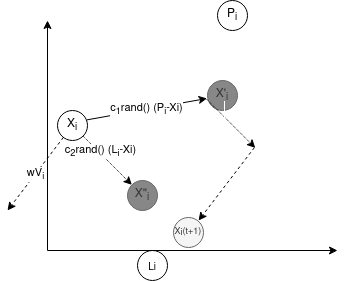
\includegraphics[]{Figures/pso2006.png} 
    \rule{35em}{0.5pt} 
    \caption[SPSO 06/07 movement]{SPSO 2006 and 2007 particle's position update. $X'_{i}$ and $X"_{i}$ are temporary point to explain the second and third terms of equation \ref{eqn:velocityInertia}.} 
    \label{fig:schemaPSO2006Update} 
\end{figure} 


\clearpage % aesthetic purpose

And while we are at it, look at the 2011 version, that you can't probably understand without the context, but eh, it's a figure to illustrate how to put some. We can see it is different than \fref{fig:schemaPSO2006Update}
\begin{figure}[H] 
    \centering 
    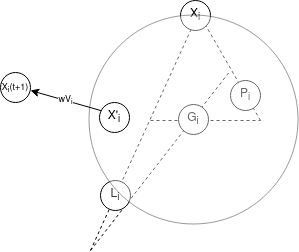
\includegraphics[]{Figures/pso2011.png} 
    \rule{35em}{0.5pt} 
    \caption[SPSO 2011 movement]{SPSO 2011 particle's position update. $X'_{i}$ is generated inside the hyper-sphere of center $G_{i}$.} 
    \label{fig:schemaPSO2011Update} 
\end{figure}

I placed my figure right after the text, but you will usually use other option to place them, such as \textit{htpb}. More info \url{https://www.overleaf.com/learn/latex/Positioning_of_Figures}. 

\begin{figure}[H] 
    \centering 
    \rotatebox{90}{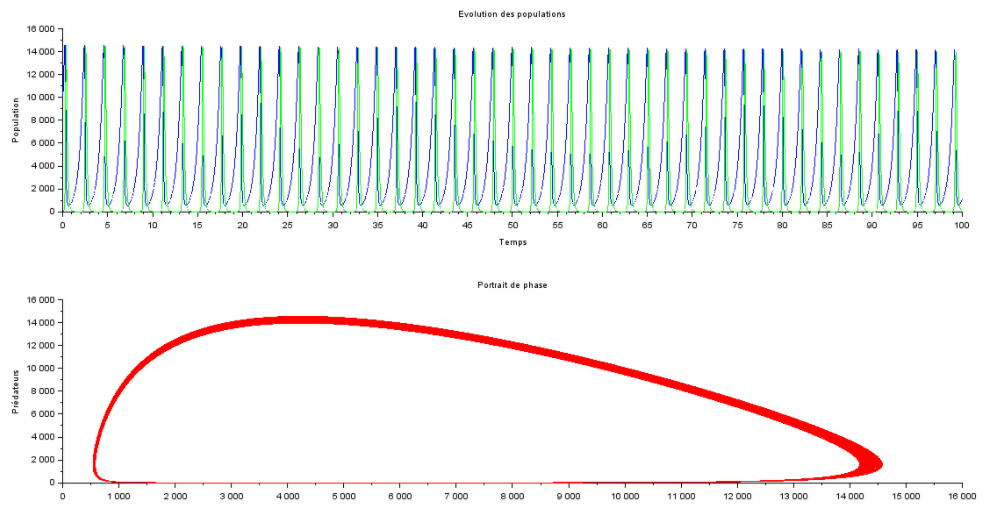
\includegraphics[width=22cm]{Figures/rk4_0-100_dt-0-0001}}
    \rule{35em}{0.5pt} 
    \caption[Sideways picture]{How to put a very big picture sideways. It is in French but who cares?} 
    \label{fig:veryBigFigure} 
\end{figure}


\begin{landscape}
\begin{figure}[!h]
    \centering
    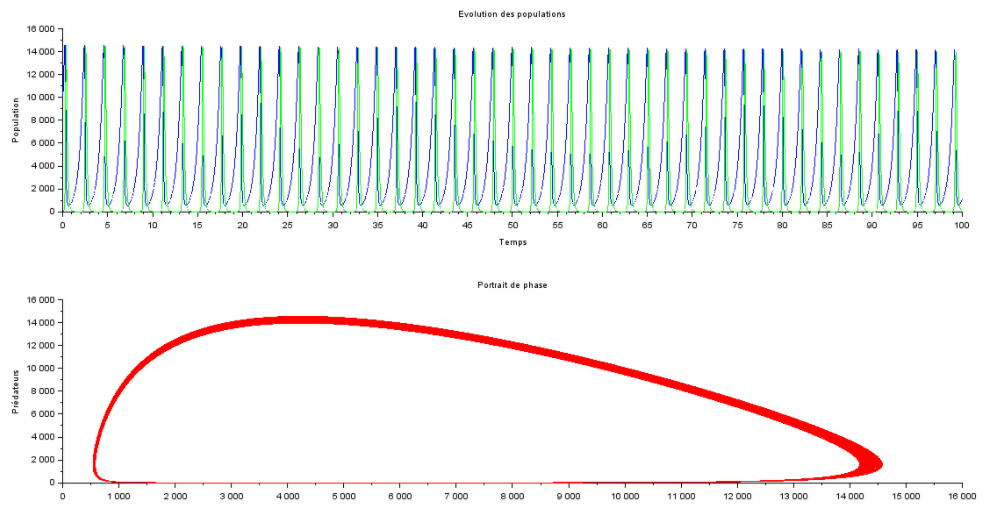
\includegraphics[width=\linewidth]{Figures/rk4_0-100_dt-0-0001}
    \caption{How to put a figure in landscape instead}
    \label{fig:verybigfigure2}
\end{figure}
\end{landscape}


\end{document}
